\documentclass[russian,utf8,14pt,simple]{eskdtext}
\usepackage[numbertop, numbercenter]{eskdplain}

% - Полуторный интервал
\renewcommand{\baselinestretch}{1.50}
% - Отступ красной строки
\setlength{\parindent}{1.25cm}	
% - Шрифт Times New Roman
\renewcommand{\rmdefault}{ftm}

% - Наименование документа
\ESKDtitle{ }
% - Обозначение документа
\ESKDsignature{ФВС КР. Х.ХХХХХХХ 001 ПЗ}
% - Наименование предприятия
\ESKDcolumnIX{ТУСУР, ФВС, КИБЭВС-1208}
% - Проверил
\ESKDchecker{Давыдова Е.М.}	
% - Литера 
\ESKDletter{У}{}{}
% - Разработал
\ESKDauthor{КИБЭВС-1208}			

% - Убирает точку в списке литературы
\makeatletter
\def\@biblabel#1{#1 }

% - ГОСТ списка литературы
\bibliographystyle{gost2008}

% - Верикальные отступы заголовков 
\ESKDsectSkip{section}{1em}{1em}
\ESKDsectSkip{subsection}{1em}{1em}
\ESKDsectSkip{subsubsection}{1em}{1em}

% - Изменение заголовков
\usepackage{titlesec}
\titleformat{\section}{\centering\normalfont\normalsize}{\thesection}{1.0em}{}
\titleformat{\subsection}{\centering\normalfont\normalsize}{\thesubsection}{1.0em}{}
\titleformat{\subsubsection}{\centering\normalfont\normalsize}{\thesubsubsection}{1.0em}{}
\titleformat{\paragraph}{\normalsize}{\theparagraph}{1.0em}{}

% - Оставим место под ТЗ 
%\setcounter{page}{4}

% - Для больших таблиц
\usepackage{longtable}
\usepackage{tabularx}
%\renewcommand{\thetable}{\thesection.\arabic{table}}

% - Используем графику в документе
\usepackage{graphicx}
\graphicspath{{images/}}
\renewcommand{\thefigure}{\thesection.\arabic{figure}}

% - Для вставки гиперссылок
\usepackage[colorlinks]{hyperref}

% - Счётчики
\usepackage{eskdtotal}

% - Для переопределения списков
\makeatletter
\renewcommand{\theenumi}{\arabic{enumi}}
\renewcommand{\labelenumi}{\theenumi)}

\renewcommand{\labelenumii}{\arabic{enumi}.\arabic{enumii}.}
\renewcommand{\labelenumiii}{\arabic{enumi}.\arabic{enumii}.\arabic{enumiii}.}
%\renewcommand{\labelenumiiii}{\arabic{enumi}.\arabic{enumii}.\arabic{enumiii}.\arabic{enumiiii}.}
\setcounter{secnumdepth}{5}

\sloppy

\begin{document}
 \section{DA}
 Анализ журналов операционных систем может помочь при решении многих задач. Примером таких задач может быть попытка восстановления системы после поломок, поиск причин неполадок системы, просмотр журналов с целью выявления активности приложений в определенные периоды и т.д. и т.п. Также, анализ журнальных файлов является неотъемлемой частью компьютерно-технических экспертиз.

При исследовании компьютеров задача анализа журнальных файлов ставится на этапе «выявление и изучение его роли в рассматриваемом деле», так как именно в журнальных файлах операционной системы хранится информация о действиях производимых на данном компьютере.

Для проведения компьютерных экспертиз существует множество специализированных программных средств, как платных так и свободно распространяемых. Примером такого средства является «OSForensics». Данный инструмент позволяет проводить множество различных исследований таких как просмотр содержимого оперативной памяти, поиск подозрительных файлов на жестком диске, составления списка программ установленных на исследуемом компьютере. Но бесплатная версия не предоставляет никаких средств по работе с журналами операционной системы. Данный факт подтолкнул к созданию собственного программного средства для проведения компьютерных экспертиз.

В данной работе описывается работа по созданию модуля для данного программного средства, позволяющего в автоматическом режиме находить, читать и конвертировать журнальные файлы операционной системы Windows XP в XML-документы, понятные для человека и легко обрабатываемые при помощи\\ электронно-вычислительных средств.

\subsubsection{Общие сведения о журнальных файлах}

В операционной системе Windows XP по умолчанию есть четыре журнала:

\begin{enumerate}
\item Журнал приложений
\item Журнал безопасности
\item Журнал установки
\item Журнал системы
\end{enumerate}

Каждый из этих журналов содержит определенный тип информации. Журналы приложений содержат информацию о запуске и остановке процессов приложений, изменении статуса каждого приложения, а также предупреждения и ошибки связанные с приложениями.

Журнал безопасности содержит информацию о входах в систему, и события связанные с безопасностью системы, например превышение количества попыток неправильно введенных подряд паролей.

Журнал установки содержит информацию об установке и обновлении компонентов системы.

Журнал системы хранит информацию о системных событиях. Например изменение схемы энергопотребления или различного рода предупреждения и ошибок.

Каждый журнал хранится в соответствующем файле с расширением .evt. Эти файлы хранятся в папке \%windows\%/system32/config. Эти файлы имеют специальную структуру.

\subsubsection{Структура журнальных файлов операционной системы Windows XP}

Все журнальные файлы операционной системы Windows XP имеют единую структуру. Файл представляет собой последовательность записей бинарных данных. Каждая запись – это структура имеющая семнадцать полей \cite{evt}.

Первые 4 байта содержат длину события в байтах, после длинны идет 4 байтный системный код сообщения. Затем 4 байтовый номер записи, после него дата создания записи, время создания, идентификатор события, тип события и так далее. Ниже приведен список полей записи, предназначенной для считывания одного события из журнального файла.

\begin{itemize}
\item uint32 Length; 
\item uint32 Reserved;
\item uint32 RecordNumber;
\item uint32 TimeGenerated;
\item uint32 TimeWritten;
\item uint32 EventID;
\item uint16 EventType;
\item uint16 NumStrings;
\item uint16 EventCategory;
\item uint16 ReservedFlags;
\item uint32 ClosingRecordNumber;
\item uint32 StringOffset;
\item uint32 UserSidLength;
\item uint32 UserSidOffset;
\item uint32 DataLength;
\item uint32 DataOffset;
\item byte[] Data.
\end{itemize}

Из сторонних источников \cite{evt} стало известно о пяти типах событий (поле EventType) (значение - тип события):

\begin{enumerate}
\item 0x0001 - Error event;
\item 0x0010 – Failure Audit event;
\item 0x0008 - Success Audit event;
\item 0x0004 - Information event;
\item 0x0002 - Warning event.
\end{enumerate}

У поля EventID удалось определить четыре значения:

\begin{enumerate}
\item 0x00 – Success;
\item 0x01 – Informational;
\item 0x02 – Warning;
\item 0x03 – Error.
\end{enumerate}

Среди множества полей записи события были выделены поля содержащие информацию о типе события, времени возникновения события и создания записи, пользователя от имени которого была сделана запись, а также поле Data - поле с бинарными данными, в которых записана подробная информация о событии.

\subsubsection{Алгоритм работы модуля}

Модуль выполняет две задачи: поиск журнальных файлов на образе диска и конвертацию каждого файла в XML-документ. Первая задача выполняется при помощи библиотек QDir и QDirIterator из Qt Framework.

QDir — библиотека позволяющая работать с конкретной директорией. Создав объект данного типа с указанием директории мы получим доступ к этой директории в программе и сможем работать в ней (просматривать содержимое; удалять, создавать или копировать файлы; создавать поддиректории). Данный объект так же поддерживать разные наборы фильтров выходных данных которые могут отсеивать ненужную информацию.

QDirIterator — библиотека, предназначенная для работы с файловой системой начиная с определенной директории как точки входа. Создав объект данного типа с указанием директории мы получим все пути которые существуют в файловой системе и начинаются с указанной директории. Данный объект поддерживает фильтрацию которая помогает выделять только необходимую информацию, исключая то, что нас не интересует, например можно вывести список только тех файлов, которые находятся в данной директории или поддиректориях, или исключить вывод символьных ссылок. Объекты данного типа используются для поиска файлов или папок на образе исследуемого диска.

Так же данные библиотеки позволяют создавать объект QFile, который позволяет работать с файлом, путь к которому передается как параметр при создании, данный объект позволяет получить базовую информацию о файле, такую как относительный или абсолютный путь до этого файла, размер файла, тип файла или его имя. Так же позволяет перемещать или копировать данный файл. Поиск работает по алгоритму представленному на рисунке \ref{evtsearch:evtSearch}.

\begin{figure}[ht]
\center{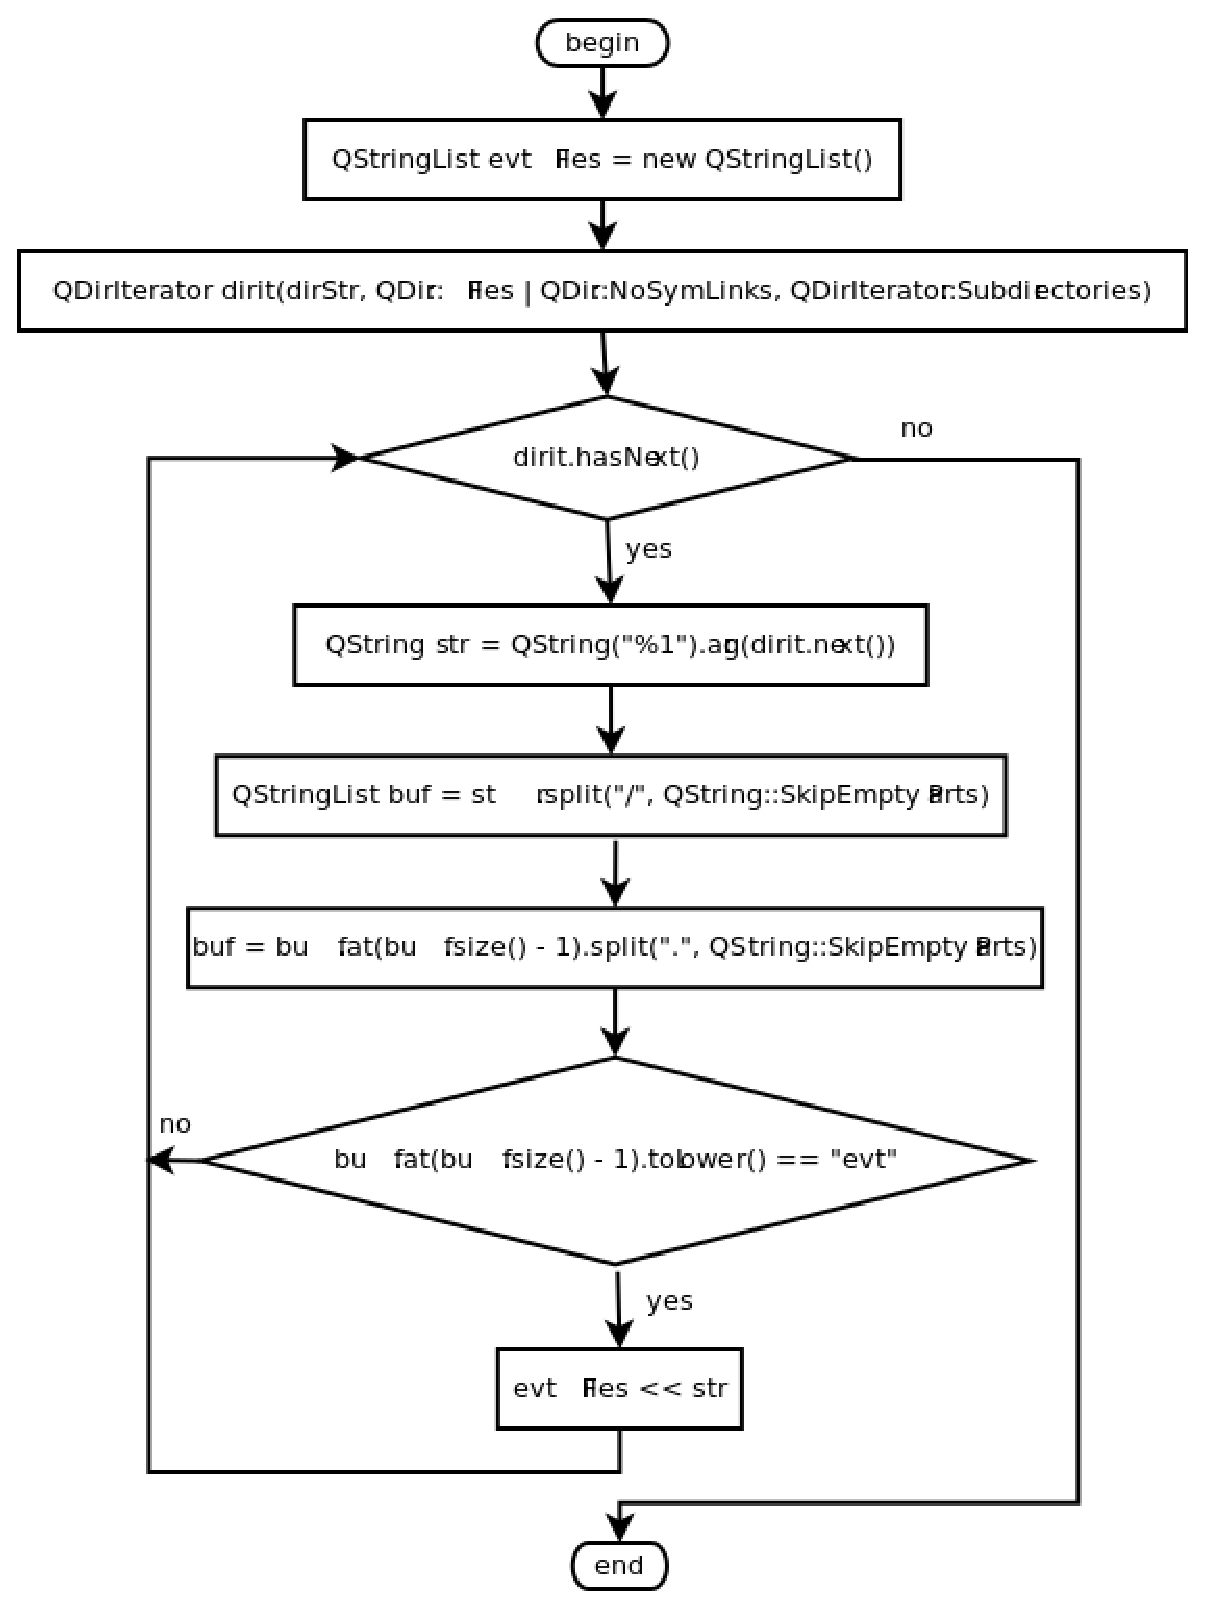
\includegraphics[width=0.6\linewidth]{evtSearch}}
\caption{Алгоритм поиска файлов с расширением *.evt}
\label{evtsearch:evtSearch}
\end{figure}

На выходе данного алгоритма мы получаем объект QStringList который содержит пути до всех найденных .evt файлов. Каждый экземпляр коллекции строк данного объекта передается в конструктор объекта winEventLog, который и конвертирует указанный файл в XML-документ. Алгоритм работы конвертора представлен на рисунке \ref{evtxml:evtToXML}.

\begin{figure}[ht]
\center{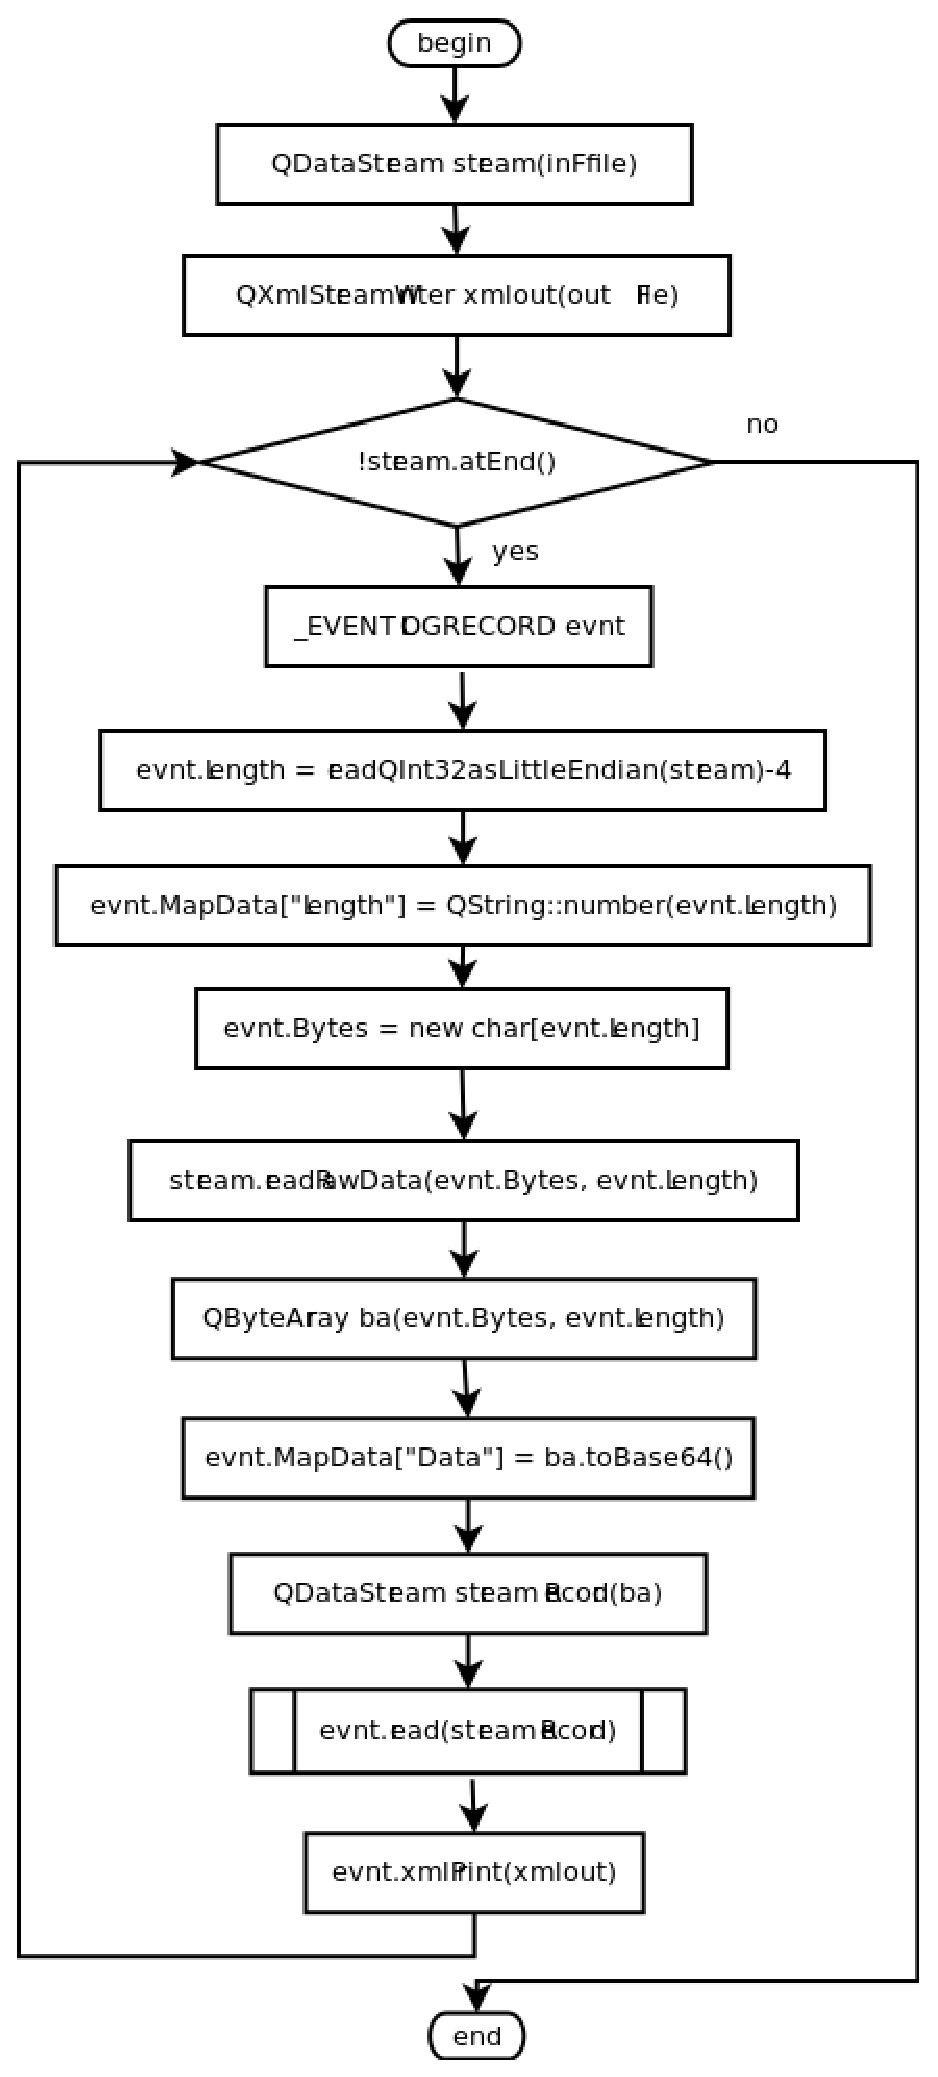
\includegraphics[width=0.4\linewidth]{evtToXML}}
\caption{Алгоритм конвертирования файлов *.evt в формат XML}
\label{evtxml:evtToXML}
\end{figure}

\end{document}
